
\subsection{Analisi} 
Periodo: dal \textbf{2021-11-19} al \textbf{2022-01-22}  \mbox{} \\ \mbox{} \\
Le precondizioni sono:
\begin{itemize}
\item Formazione del gruppo;
\item Assegnazione capitolato\glo{} d’appalto C4.
\end{itemize}  \mbox{} \\
Le postcondizioni sono:
\begin{itemize}
\item Redazione dei documenti:
\begin{itemize}
	\item Norme di Progetto;
	\item Piano di Progetto;
	\item Piano di Qualifica;
	\item Analisi dei Requisiti;
	\item Glossario.
\end{itemize}
\item Verifica di quanto redatto.
\end{itemize}

\subsubsection{Attività}

Le attività che compongono l’analisi sono composte dai diversi documenti:

\begin{itemize}
\item \textbf{\textit{Norme di Progetto}}: in questo documento vengono definite tutte le regole a cui il gruppo DreamTeam dovrà attenersi per la stesura degli altri documenti. Inoltre, in questo documento vengono indicati anche i vari strumenti da utilizzare per realizzare il progetto ed i vari diagrammi (ad esempio, UML\glo{});  
\item \textbf{\textit{Piano di Progetto}}: il presente documento illustra un prospetto di pianificazione dettagliata, con attività e compiti, a cui il gruppo DreamTeam dovrà attenersi per lo sviluppo del progetto;
\item \textbf{\textit{Piano di Qualifica}}: che ha lo scopo di fissare standard ed obiettivi che permettano di quantificare la qualità dei processi e dei prodotti da rispettare durante tutta la durata del progetto;
\item \textbf{\textit{Analisi dei Requisiti}}: all’interno vengono spiegati i diversi requisiti che dovrà avere e rispettare il prodotto che verrà sviluppato. Per comprendere meglio i vari requisiti, verranno illustrati anche i diversi casi d’uso con dei diagrammi UML;
\item \textbf{\textit{Glossario}}: al suo interno si possono trovare tutte le parole chiave utilizzate nei vari documenti e che potrebbero risultare ambigue, per ciascuna parola viene data una descrizione concisa.
\end{itemize}

\subsubsection{Periodi}

Questa fase è stata suddivisa in tre periodi distinti, che andremo ad analizzare in seguito.

\subsubsubsection{I Periodo}

\textbf{2021-11-19 – 2021-11-29}: in questo primo periodo viene definito lo scheletro dei documenti, le regole di base delle attività del gruppo e lo strumento per gestire i ticket\glo{}. Inoltre, in questo periodo vengono scritti i primi verbali interni delle riunioni svolte con tutti i componenti del gruppo.

\subsubsubsection{II Periodo}

\textbf{2021-11-30 – 2022-01-09}: questo periodo è il più ricco, in quanto vengono scritti tutti i documenti, partendo dalle \textit{Norme di Progetto}. Seguono \textit{Analisi dei Requisiti}, \textit{Piano di Progetto} e \textit{Piano di Qualifica}, oltre al \textit{Glossario} nel quale vengono inserite parole chiave presenti nei documenti appena citati. In questo secondo periodo viene fatta anche una riunione con il proponente e vengono svolte le attività di formazione delle varie tecnologie, che dovranno essere utilizzati per lo sviluppo del Proof of Concept e dell’intero progetto. È stato stabilito che dovrà essere fatta almeno una riunione interna, con tutti i componenti del gruppo, a settimana. \\
Infine, iniziano le prime attività di verifica incrementale per i documenti in corso di stesura. 

\subsubsubsection{III Periodo}

\textbf{2022-01-10 – 2022-01-22}: questo terzo periodo è dedicato alla verifica di coerenza e coesione complessiva dei documenti, oltre all’inserimento di alcuni termini mancanti nel glossario. Oltre a ciò, vengono adattati tutti i documenti rispetto quanto stabilito nelle \textit{Norme di Progetto}.

\begin{figure}[H]
\centering
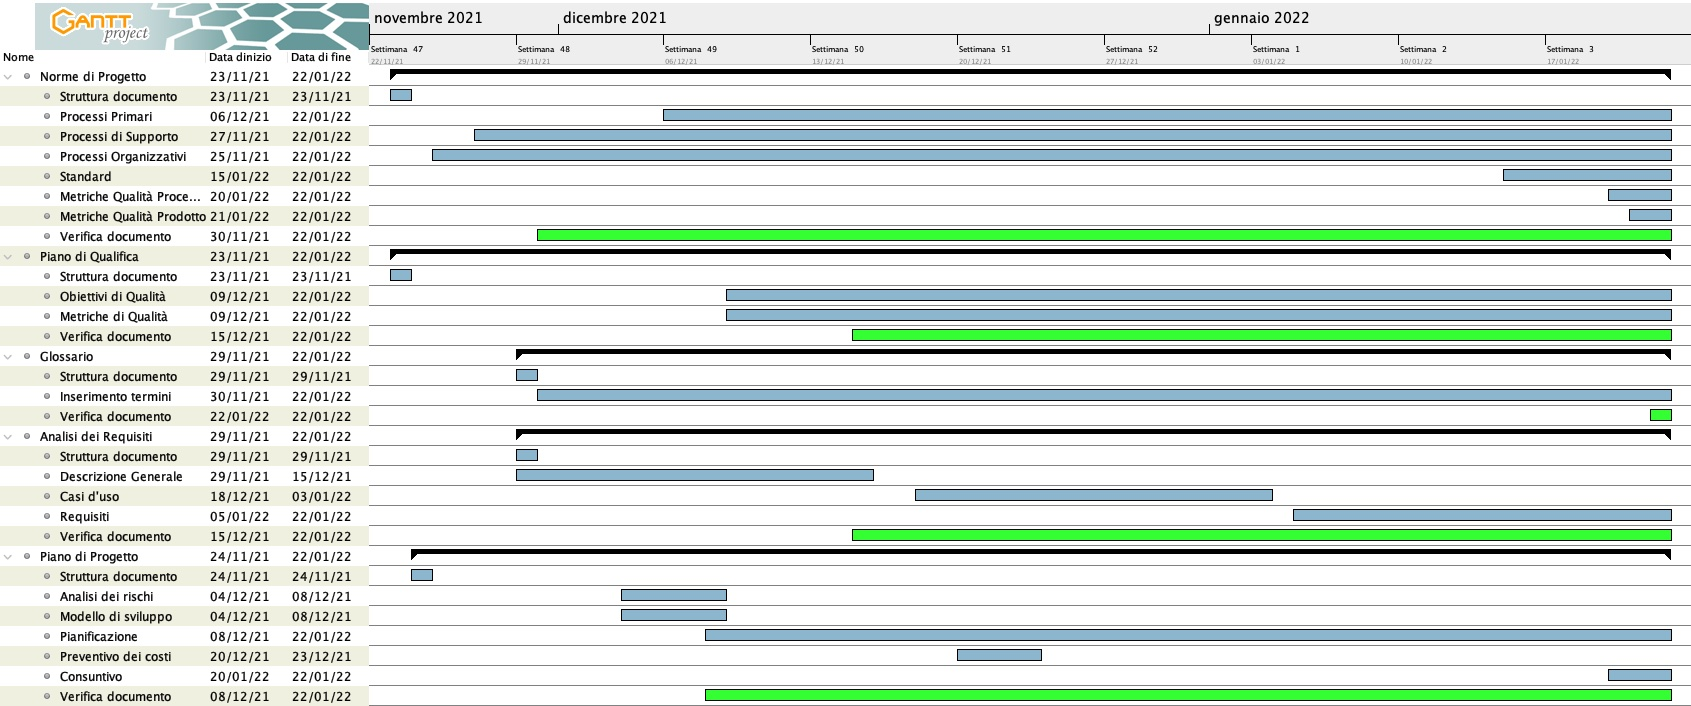
\includegraphics[scale=0.35]{Sezioni/gantt/Analisi.png}
\caption{Diagramma di Gantt\glo{} - Analisi}
\end{figure}
